%% ----------------------------------------------------------------
%% Progress.tex
%% ---------------------------------------------------------------- 
\documentclass[sotoncolour]{uosprogress}    % Use the progress Style with custom link colour
\graphicspath{{./Figures/}}   % Location of your graphics files
\usepackage[square, numbers]{natbib}            % Use Natbib style for the refs.
\usepackage[final]{pdfpages}
\hypersetup{colorlinks=true}   % Set to false for black/white printing
%% ----------------------------------------------------------------
%% Definitions.tex
%% ---------------------------------------------------------------- 
\newcommand{\BibTeX}{{\rm B\kern-.05em{\sc i\kern-.025em b}\kern-.08em T\kern-.1667em\lower.7ex\hbox{E}\kern-.125emX}}

%% People
\newcounter{address}
\setcounter{address}{1}
\renewcommand{\theaddress}{\textsuperscript{\fnsymbol{address}}}
\newcommand{\address}[1]{\refstepcounter{address}\theaddress#1\\}
\newcommand{\Name}[3]{\texorpdfstring{\href{mailto:#3}{#2}#1}{#2}\xspace}
\newcommand{\SteveRGunn}[1]{\Name{#1}{Steve R. Gunn}{S.R.Gunn@ecs.soton.ac.uk}}

%% Dingbats
\newcommand{\tick}{\ding{51}}
\newcommand{\cross}{\ding{55}}

%% Calculus
\newcommand{\pd}[2]{\ensuremath{\frac{\partial #1}{\partial #2}}\xspace}
\newcommand{\fd}[2]{\ensuremath{\frac{d #1}{d #2}}\xspace}
\newcommand{\dint}{\ensuremath{\int\!\!\!\int}\xspace}
\newcommand{\tint}{\ensuremath{\int\!\!\!\int\!\!\!\int}\xspace}

%% Math Sets
\newcommand{\Q}[1]{\ensuremath{\mathbb{#1}}\xspace}
\newcommand{\R}{\Q{R}}

%% Matrix, Vector
\newcommand{\V}[1]{\ensuremath{\boldsymbol{#1}}\xspace}
\newcommand{\M}[1]{\ensuremath{\boldsymbol{#1}}\xspace}
\newcommand{\0}{\V{0}}
\newcommand{\1}{\V{1}}
\newcommand{\I}{\M{I}}

%% Math Functions
\newcommand{\F}[1]{\ensuremath{\mathrm{#1}}\xspace}
\newcommand{\sgn}{\F{sgn}}
\newcommand{\tr}{\F{trace}}
\newcommand{\diag}{\F{diag}}

%% Math Names
\newcommand{\N}[1]{\ensuremath{\mathit{#1}}\xspace}

%% Data
\newcommand{\mc}[1]{\ensuremath{\mathcal{#1}}\xspace}
\newcommand{\Hyp}{\mc{H}}
\newcommand{\D}{\mc{D}}

%% Kernel
\newcommand{\K}{\M{K}}
\newcommand{\eins}{\texorpdfstring{\ensuremath{\epsilon}}{\textepsilon}-insensitive\xspace}
\newcommand{\e}{\ensuremath{\epsilon}\xspace}
\newcommand{\Bxi}{\ensuremath{\boldsymbol{\xi}}\xspace}
\newcommand{\Kanova}{\ensuremath{\mathit{K_{ANOVA}}}\xspace}
\newcommand{\Kspline}{\ensuremath{\mathit{K_{spline}}}\xspace}

%% Bayesian
\newcommand{\MP}{\ensuremath{\mathit{{\scriptscriptstyle \hspace{-1.5pt}M\hspace{-1.5pt}P}}}\xspace}
\newcommand{\ML}{\ensuremath{\mathit{{\scriptscriptstyle \hspace{-1.5pt}M\hspace{-1.5pt}L}}}\xspace}
\newcommand{\Qw}{\ensuremath{Q_{\w}(\w)}\xspace}
\newcommand{\Qa}{\ensuremath{Q_{\Ba}(\Ba)}\xspace}
\newcommand{\Qb}{\ensuremath{Q_{\beta}(\beta)}\xspace}
\newcommand{\wMPab}{\ensuremath{\w_{\MP|\bar {\Ba},\bar \beta}}\xspace}
\newcommand{\wMP}{\ensuremath{\w_{\MP}}\xspace}
\newcommand{\yMP}{\ensuremath{y_{\MP}}\xspace}
\newcommand{\BaMP}{\ensuremath{\Ba_{\hspace{1pt}\MP}}\xspace}
\newcommand{\aMP}{\ensuremath{\alpha_{\hspace{1pt}\MP}}\xspace}
\newcommand{\bMP}{\ensuremath{\beta_{\hspace{1pt}\MP}}\xspace}
\newcommand{\Sab}{\ensuremath{\M{\Sigma}_{\bar \Ba,\bar \beta}}\xspace}
\newcommand{\Ba}{\ensuremath{\boldsymbol{\alpha}}\xspace}
\newcommand{\Bb}{\ensuremath{\boldsymbol{\beta}}\xspace}
\newcommand{\Bm}{\ensuremath{\boldsymbol{\mu}}\xspace}
\newcommand{\BL}{\ensuremath{\boldsymbol{\Lambda}}\xspace}
\newcommand{\BPhi}{\ensuremath{\boldsymbol{\Phi}}\xspace}
\newcommand{\SMP}{\ensuremath{\M{\Sigma}_{\MP}}\xspace}

\newcommand{\Pa}{\ensuremath{P(\alpha|\mathcal{H})}\xspace}
\newcommand{\Pb}{\ensuremath{P(\beta|\mathcal{H})}\xspace}
\newcommand{\Pab}{\ensuremath{P(\alpha,\beta|\mathcal{H})}\xspace}
\newcommand{\Pw}{\ensuremath{P(\w|\mathcal{H})}\xspace}
\newcommand{\PD}{\ensuremath{P(\D|\mathcal{H})}\xspace}
\newcommand{\PwIa}{\ensuremath{P(\w|\alpha,\mathcal{H})}\xspace}
\newcommand{\PDIwb}{\ensuremath{P(\D|\w,\beta,\mathcal{H})}\xspace}
\newcommand{\PDwab}{\ensuremath{P(\D,\w,\alpha,\beta|\mathcal{H})}\xspace}
\newcommand{\PDIw}{\ensuremath{P(\D|\w,\mathcal{H})}\xspace}
\newcommand{\PwID}{\ensuremath{P(\w|\D,\mathcal{H})}\xspace}
\newcommand{\PwabID}{\ensuremath{P(\w,\alpha,\beta|\D,\mathcal{H})}\xspace}

\newcommand{\PanH}{\ensuremath{P(\alpha)}\xspace}
\newcommand{\PbnH}{\ensuremath{P(\beta)}\xspace}
\newcommand{\PabnH}{\ensuremath{P(\alpha,\beta)}\xspace}
\newcommand{\PwnH}{\ensuremath{P(\w)}\xspace}
\newcommand{\PDnH}{\ensuremath{P(\D)}\xspace}
\newcommand{\PwIanH}{\ensuremath{P(\w|\alpha)}\xspace}
\newcommand{\PDIwbnH}{\ensuremath{P(\D|\w,\beta)}\xspace}
\newcommand{\PDwabnH}{\ensuremath{P(\D,\w,\Ba,\beta)}\xspace}
\newcommand{\PDIwnH}{\ensuremath{P(\D|\w)}\xspace}
\newcommand{\PwIDnH}{\ensuremath{P(\w|\D)}\xspace}
\newcommand{\PwabIDnH}{\ensuremath{P(\w,\alpha,\beta|\D)}\xspace}

\newcommand{\PDwBab}{\ensuremath{P(\D,\w,\Ba,\beta|\mathcal{H})}\xspace}
\newcommand{\PwIBa}{\ensuremath{P(\w|\Ba,\mathcal{H})}\xspace}
\newcommand{\PBab}{\ensuremath{P(\Ba,\beta|\mathcal{H})}\xspace}
\newcommand{\PwBabID}{\ensuremath{P(\w,\Ba,\beta|\D,\mathcal{H})}\xspace}

\newcommand{\PBanH}{\ensuremath{P(\Ba)}\xspace}
\newcommand{\PwIBanH}{\ensuremath{P(\w|\Ba)}\xspace}

%% Snakes
\newcommand{\Esnake}{\ensuremath{\mathit{E_{snake}}}\xspace}
\newcommand{\Eimage}{\ensuremath{\mathit{E_{image}}}\xspace}
\newcommand{\Econt}{\ensuremath{\mathit{E_{cont}}}\xspace}
\newcommand{\Ecurv}{\ensuremath{\mathit{E_{curv}}}\xspace}
\newcommand{\Eint}{\ensuremath{\mathit{E_{int}}}\xspace}
\newcommand{\Eext}{\ensuremath{\mathit{E_{ext}}}\xspace}
\newcommand{\Eterm}{\ensuremath{\mathit{E_{term}}}\xspace}
\newcommand{\Eline}{\ensuremath{\mathit{E_{line}}}\xspace}
\newcommand{\Eedge}{\ensuremath{\mathit{E_{edge}}}\xspace}
\newcommand{\Econ}{\ensuremath{\mathit{E_{con}}}\xspace}
\newcommand{\Eangle}{\ensuremath{\mathit{E_{angle}}}\xspace}
\newcommand{\Elshape}{\ensuremath{\mathit{E_{lshape}}}\xspace}
\newcommand{\Eedgedir}{\ensuremath{\mathit{E_{edgedir}}}\xspace}
\newcommand{\Emodel}{\ensuremath{\mathit{E_{model}}}\xspace}
\newcommand{\wte}{\ensuremath{\mathit{w_{term}}}\xspace}
\newcommand{\wli}{\ensuremath{\mathit{w_{line}}}\xspace}
\newcommand{\wed}{\ensuremath{\mathit{w_{edge}}}\xspace}
\newcommand{\wco}{\ensuremath{\mathit{w_{con}}}\xspace}

%% Environments
\newcounter{alg}
\newenvironment{algorithm}[1]
{
    \stepcounter{alg}
    \begin{table}[htb]
    \centering
    \begin{tabular}[t]{ll}
    \hline&\\
    \multicolumn{2}{l}{\bf Algorithm \arabic{alg}: #1}\\&\\
} {
    &\\
    \hline
    \end{tabular}
    \end{table}
}
            % Include your abbreviations
%% ----------------------------------------------------------------
%% --------------------THESIS/DOC INFORMATION ---------------------
\faculty     {Faculty of Physical Sciences and Engineering}
\FACULTY     {\MakeUppercase{\facname}}
\department  {Electronics and Computer Science}
\DEPARTMENT  {\MakeUppercase{\deptname}}
\group       {}
\GROUP       {\MakeUppercase{\groupname}}
\title      {A Deep Learning Method for Traffic Prediction}
\authors    {\texorpdfstring
            {\href{mailto:yz25g21@soton.ac.uk}{Yanzhe (Solomon) Zhang}}
            {}
            }
\addresses  {\groupname\\\deptname\\\univname}
\date       {\today}
\supervisor {Professor Lie-Liang Yang}
\examiner   {}
%% Optional Fields TODO: Replace these fields with your own data

\qualifications{MEng}
\subject    {Part III Individual Project}
\keywords   {}

\begin{document}

%% ------------------ FRONT MATTER ORGANISATION -------------------
\frontmatter
\maketitle
\begin{abstract}
This is the progress report of the Part III Project. 

In contemporary urban environments, efficient urban mobility is imperative for daily routines. 
Traffic congestion stands as a pervasive challenge in urban areas, leading to delays, frustration, and inefficiencies in transportation systems. 
This project aims to explore traffic prediction using deep learning techniques, specifically recurrent neural networks (RNNs), to provide accurate insights into future traffic conditions.

As reached halfway through the project, the dataset had been found, data had been preprocessed, and an LSTM model had been constructed. 
In the next term, it is planned to optimize the hyperparameters of the model and add spatial aspects to it. 

\end{abstract}

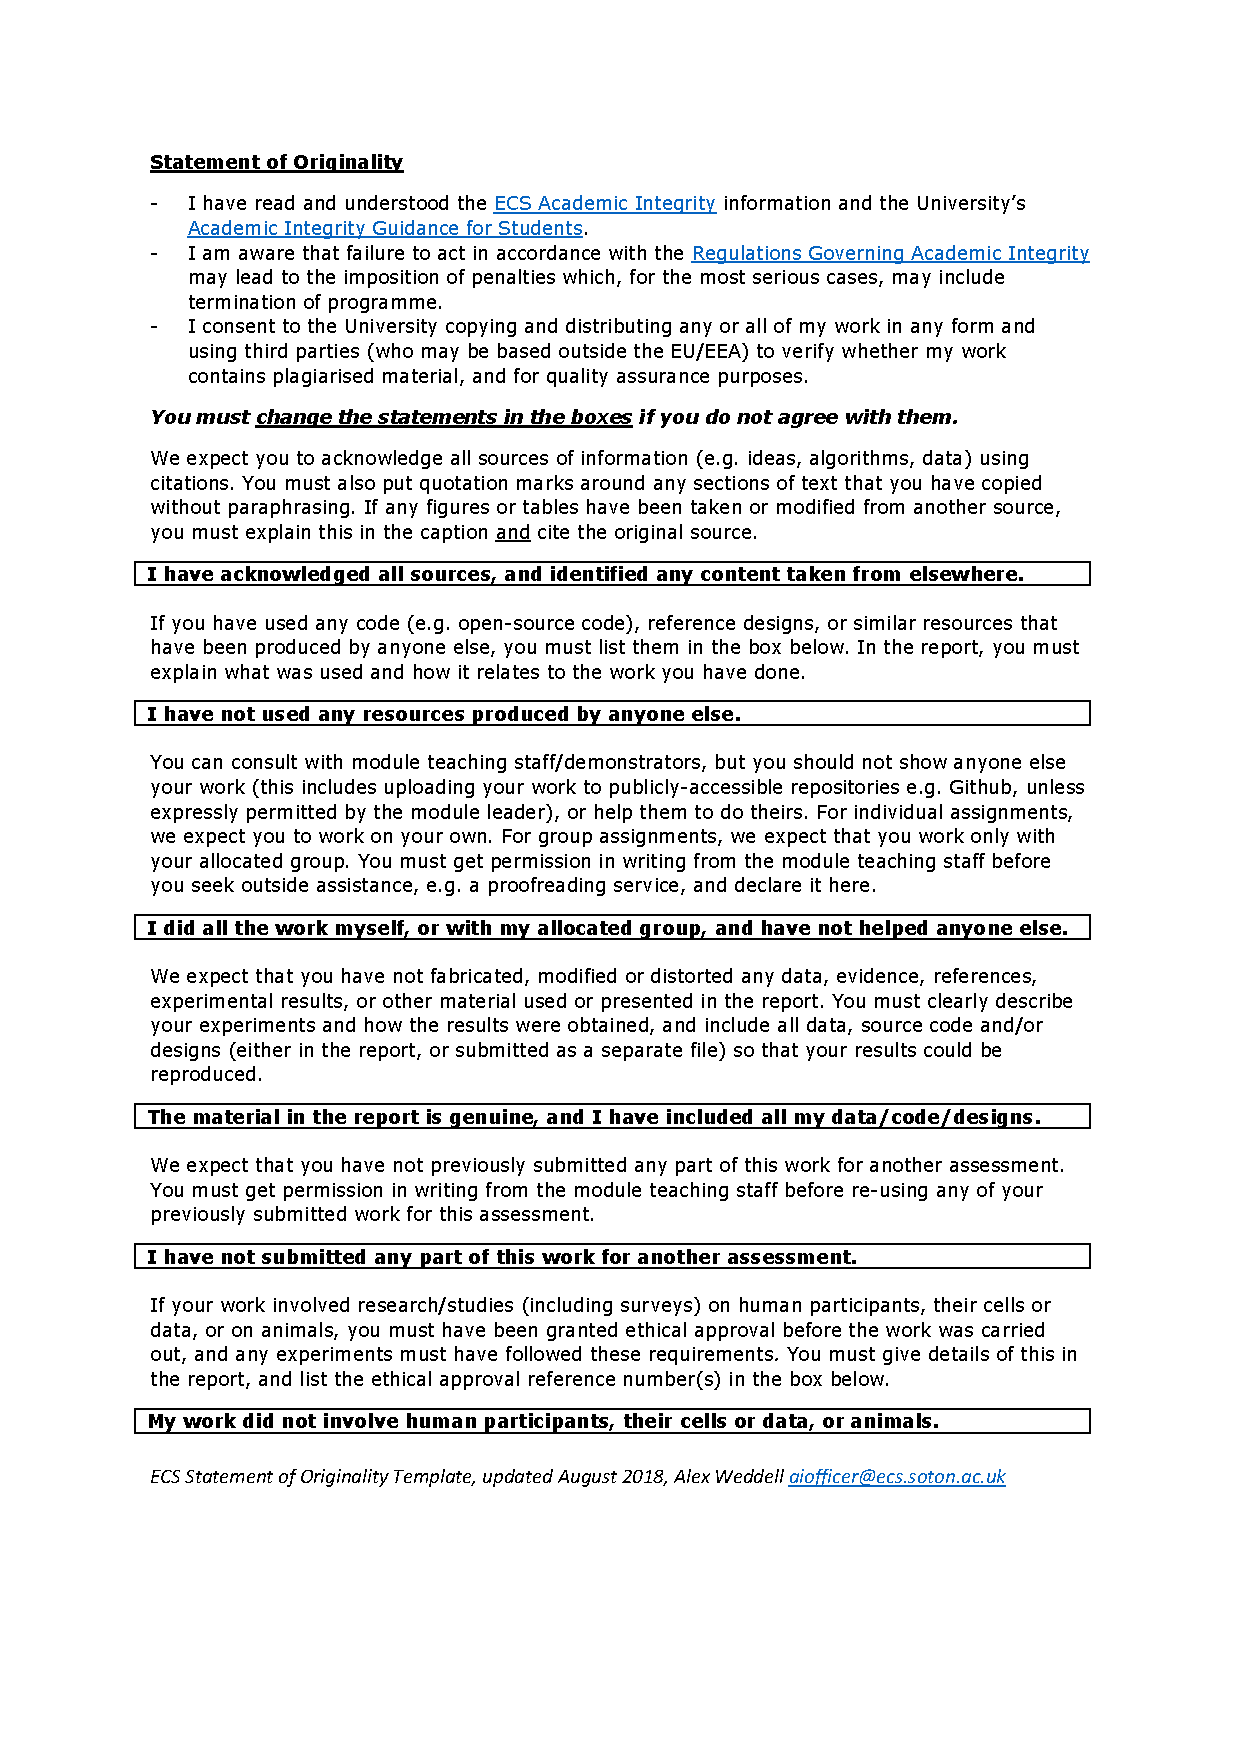
\includepdf{ai_statement.pdf}
% \acknowledgements

\let\cleardoublepage\clearpage

\pdfbookmark[0]{\contentsname}{toc} % Add pdf bookmark for contents page for navigation

\tableofcontents
% \listoffigures
% \listoftables

%% The List of listings does not, by default, appear in the ToC, so....
% \addtotoc{Listings}
% \lstlistoflistings
% \listofaddmaterial
% \addtolom{Material Name e.g Map}
% \addtolom{Material Name e.g CD}
% \addtolom{Test Material}

%%Lightweight Definitions and Abbreviations see package:nomencl for alternative
%% Include if relevant to discipline
% \listofsymbols{ll}{$w$ & The weight vector\\$\S$ & If relevant to discipline}

\let\cleardoublepage\clearpage

%% ------------------ MAIN MATTER (CONTENT) ----------------------
\mainmatter

%% ----------------------------------------------------------------
%% Introduction.tex
%% ---------------------------------------------------------------- 
\chapter{Introduction} \label{Chapter:Introduction}

In modern, fast-paced lives, urban mobility is an integral aspect that significantly impacts our daily routines. 
One of the most pervasive challenges in urban areas is the issue of traffic congestion, causing delays, frustration, and inefficiencies in transportation systems. 
This poses high requirements for traffic management and navigation systems addressing these problems. 
In the topic of traffic management and planning, accurate prediction of vehicles and proactively suggesting optimal routes in urban road networks is one of the important tasks to improve traffic efficiency and safety.
This project seeks to explore the realm of traffic prediction, employing deep learning techniques to provide accurate insights into future traffic conditions. 

The project focuses on near-future predictions, more specifically, predicting the traffic condition in half-hour advance. 
There are two approaches to the aims that are covered, one is to train a model for a single location, predicting traffic at individual points on the map.
This is referred to as the Localised designs in this report. 
By focusing on specific locations within the map, localised predictions offer detailed insights into traffic patterns and congestion levels at particular points of interest. 
It allows for targeted interventions and optimizations at specific locations. It can also provide a source for navigation apps with real-time traffic information and suggest routes to avoid congested areas. 

The other approach is to consider an area of roads as a whole, predicting the traffic for all roads of that area at the same time, namely the Globalised designs. 
It offers a holistic view of traffic conditions across a certain area, enables city authorities to manage traffic flow, and implements politics to alleviate congestion on a broader scale.
%% ----------------------------------------------------------------
%% Background.tex
%% ---------------------------------------------------------------- 
\chapter{Theoretical Background} \label{Chapter:Background}

\section{Machine Learning}

Machine learning focuses on developing algorithms and models that enable computers to learn patterns from data and make predictions or decisions without being explicitly programmed for the task \cite{Murphy}. 
The use of statistical techniques such as linear regression allows it to improve its performance over time as it is exposed to more information. 
There are three commonly used machine learning approaches \cite{Bishop} including supervised learning, where the algorithm is trained on labeled data; 
unsupervised learning, where the algorithm discovers patterns in unlabeled data; and reinforcement learning, where the algorithms learn through trial and error based on feedback from its actions.

\subsection{Performance Measure}

In both machine learning and deep learning, the cost function is often the target to minimize. This function measures how well a model is performing on the training data.
In this project, mean squared error (MSE) and mean absolute percentage error (MAPE) have been considered. The functions of the two indicators are shown below:

\begin{gather}
    \mathrm{MSE} = \frac{1}{n}\sum_{i=1}^{n}(\hat{y_i} -y_i)^2 
\end{gather}

MSE calculates the square of the difference between the predicted value $\hat{y_i}$ and the actual value $y_i$, and takes the mean of it \cite{Bishop}. 
The value is in the range of $[0, +\infty)$, when the predicted value equals the real value, MSE is 0. As the difference gets larger, MSE increases. 

\begin{gather}
    \mathrm{MAPE} = \frac{100\%}{n} \sum_{i=1}^{n} \left | \frac{\hat{y_i}-y_i}{y_i} \right | 
\end{gather}

Instead of the actual value of the loss, MAPE is more focused on percentage \cite{Hyndman}. The range of MAPE is also $[0, +\infty)$, where a 0\% MAPE means a perfect match, and above 100\% would be considered as bad. 
Note that when the real value is in the denominator, which means it is not useable for any data set that contains a real value of 0.

\subsection{Gradient Descent}

Gradient descent is an optimization algorithm used to minimize the cost function iteratively. The gradient or derivative of the cost function at a point tells the direction of the steepest increase of the function. 
Hence if the parameters are updated in the opposite direction of the gradient, the model will be closer, and potentially reach the mimimum cost. 
The size of the the step of each update is controlled by the learning rate. 

For example in linear regression, we shell fit the data using a polynomial function \cite{Bishop}: 

\begin{gather}
    \hat{y}(x, \mathbf{w}) = \omega _0 + \omega _1x^1 + \omega _2x^2 + \dots +\omega _nx^n = \sum_{i=0}^{n}\omega _ix^i 
\end{gather}

Where the function has an order of n, with parameters $\omega_i$ controlling each term. These parameters are also denoted as vector $\mathbf{w}$ for future convenience.

The cost function using MSE hence can be denoted as:

\begin{gather}
    \mathrm{MSE} = \frac{1}{n}\sum_{i=1}^{n}(\hat{y}(x_i, \mathbf{w}) - y_i)^2 
\end{gather}

A step of gradient descent can be represented as below, repeat the process until achieving a certain level of accuracy, or other convergence criteria. 

\begin{gather}
    \mathbf{w}_{new} = \mathbf{w}_{old} - \alpha \times \nabla(\mathrm{MSE})
\end{gather}

\subsection{One-hot Encoding}

Sometimes the data used in machine learning contains categorical variables, which represent categories or labels, such as colors and the class of a road.
Each value of these variables is independent, the size does not matter. To let the model understand this better, one-hot encoding could be introduced.

One-hot encoding is a technique used to represent those categorical variables as binary vectors. The length of the vectors is equal to the number of unique categories,
and each position in the vector corresponds to a specific category. If the data is in a category, the corresponding position is set to be 1, otherwise, fill with 0. 
With this implemented, each category is treated as an independent entity and does not impose any ordinal relationship. 

\section{Deep Learning}

Deep learning is a subset of machine learning, which includes the use of neural networks. It is designed to solve complex problems with large datasets. 
Popular deep learning architectures include convolutional neural networks (CNNs), recurrent neural networks (RNNs), and transformers.

\subsection{Neural Network}

At the core of deep learning are artificial neural networks (ANN), which are inspired by the structure and functioning of the human brain. 
The structure of a neural network is illustrated in \fref{Figure:ANN-structure}. It is composed of layers of interconnected nodes (neurons). 
The input layer is where the data is fed into the network, and the output layer produces the final result. Between the input and output layers, there are one or more hidden layers 
each node in the hidden layers has a usually non-linear activation function. Section \ref{Section:activation} talks more about them. Lines between layers are linear transformations, 
with the parameter vector $\mathbf{w}$, and bias $\mathrm{b}$. 

\begin{figure}[!htb]
    \centering
    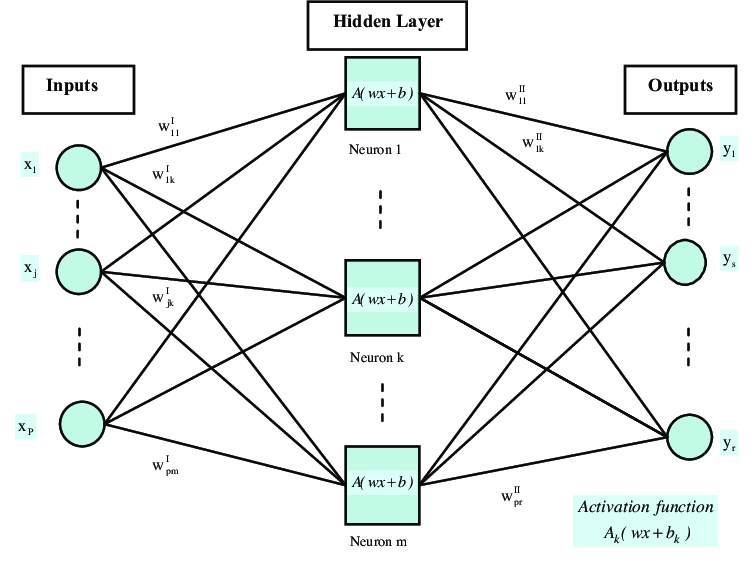
\includegraphics[width=12cm]{ANN-structure}
    \caption{A simple ANN structure with one hidden layer (Adapted from \cite{Kocadağlı})}
    \label{Figure:ANN-structure}
\end{figure}

What the network trying to do is the same as machine learning: find a function that best fits the data, so it can make predictions. The process could be expressed as:

\begin{gather}
    \mathbf{y} =\mathbf{w}^{II} \times A_k (\mathbf{w^Ix} + b^I_k)+ b^{II}
\end{gather}

The inputs fed into the network first go through a linear transformation and then map to an activation function. At last, go through a linear transformation again and output. 
By altering the parameters, it is possible to construct any curve. 

Deep learning emphasizes the use of deep neural networks, which means networks with multiple hidden layers. These networks are capable of learning complex datasets with non-intuitive 
characteristics. The depth allows the network to automatically learn features at different levels of abstraction.

Backpropagation is a key used in training deep neural networks. It is a supervised learning algorithm that adjusts the parameters $\mathbf{w}$
by propagating the error backward from the output layer to the input layer. This allows the network to update parameters to optimize predictions. 
Gradient descent is one of the backpropagation methods. Knowing the error from prediction, it measures which connection in the hidden layer.

\subsection{Activation Functions} \label{Section:activation}

The choice of activation function is vital in neural networks by introducing non-linearity into the model \cite{activation}. 
It enables the network to learn complex patterns and relationships in the data. 

\subsubsection{Rectified Linear Unit (ReLU)}

ReLU is one of the most commonly used activation functions. It replaces all negative values in the inputs with zero, which can be represented by: 
\begin{gather}
    f(x) = \mathrm{max}(0, x) 
\end{gather}

During the training, it will not activate all neurons at the same time, which gives an advantage that it is computationally efficient.
However, when $x < 0$, the gradient is zero. As training progresses, neurons may become inactive and weights fail to update.
To solve this problem, a variant of ReLU, Leaky ReLU, could be used instead. Leaky ReLU allows a small, non-zero gradient when the input is negative.

\begin{gather}
    f(x) = \mathrm{max}(\alpha x, x) 
\end{gather}

Where $\alpha$ is a small positive constant. A plot of both functions is shown in \fref{Figure:ReLUplots}

\begin{figure}[!htb]
    \centering
    \subcaptionbox{ReLU}{
        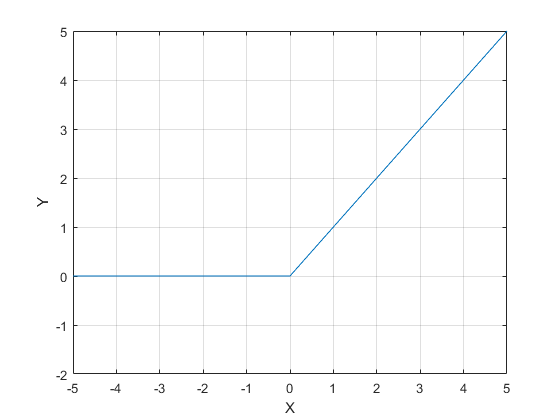
\includegraphics[width=6.5cm]{ReLU}
        \label{Figure:ReLUplots:ReLU}
    }
    \subcaptionbox{Leaky ReLU}{
        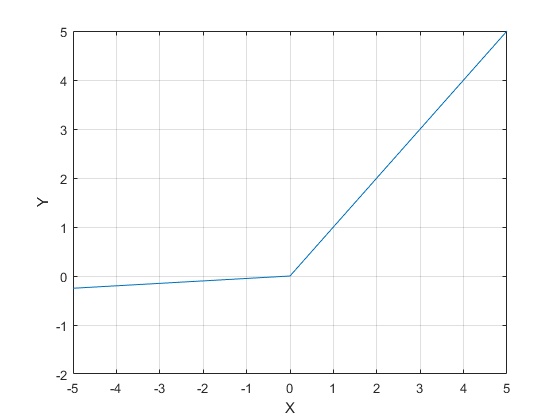
\includegraphics[width=6.5cm]{LeakyReLU}
        \label{Figure:ReLUplots:LeakyReLU}
    }
    \caption{ReLU activation functions}
    \label{Figure:ReLUplots}
\end{figure}

It is also possible to use the exponential linear units (ELU) to address the problem of inactive neurons. 
It uses $e^x-1$, which gives a similar curve, but has a small negative value at $x < 0$. 

\subsubsection{Other Functions}

There are many other activation functions such as sigmoid, hyperbolic tangent (Tanh), Softmax, etc.
Those are suitable for different purposes. For example, sigmoid have a limited output range, suitable to use before output. 
However, the curve gets too smooth at two ends, which causes a low learning efficiency. It is more used in classification problems. 

\section{Recurrent Neural Networks (RNNs)}

RNNs are a type of ANN designed for sequence data where the order of the data points is crucial \cite{lipton2015critical}. 
This makes RNN a good approach for this project. Similar to the simple ANN, RNN is constructed by multiple RNN cells. The formula of each cell is given by:

\begin{gather}
    \mathbf{h}_t = A (\mathbf{w^Ix}_t + \mathbf{w^{II}h}_{t-1} + b)
\end{gather}

Where $\mathbf{x}_t$ is the input at time $t$, $\mathbf{h}_t$ is the output at $t$, hence, $\mathbf{h}_{t-1}$ is the output at time $t-1$. 
Everything else is the same as the simple ANN. The essence of RNN is that the output of the current moment will take place in the calculation 
of the next moment as one of the inputs. \fref{Figure:RNN-structure} illustrates the idea of RNN.

\begin{figure}[!htb]
    \centering
    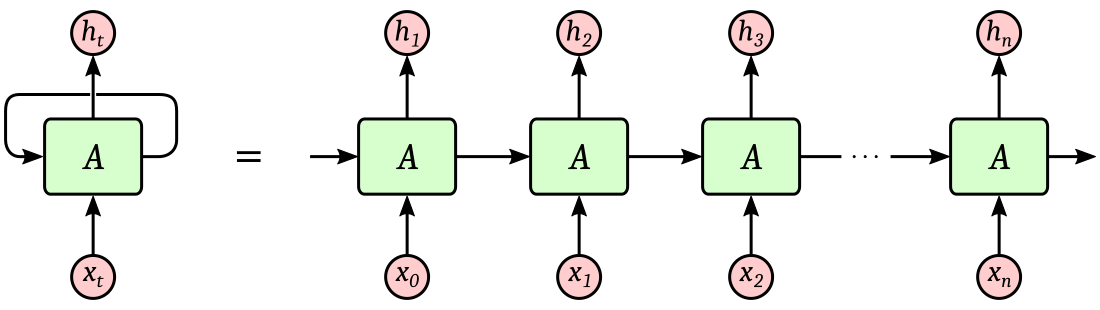
\includegraphics[width=12cm]{rnn}
    \caption{RNN as a neural network very deep in time (Adapted from \cite{rnnplot})}
    \label{Figure:RNN-structure}
\end{figure}

RNNs are susceptible to the vanishing/exploding gradient problem \cite{ribeiro2020exploding}. 
Since the RNN uses the backpropagation to minimize the cost function, and the error has been calculated from outputs going back through the network to update the weights, 
those weights in the feedback loop ($\mathbf{w_{rec}}$) are multiplied a lot of times during the backpropagation. 
If $\mathbf{w_{rec}} < 1$, the gradient will be vanishing, since it approaches 0. In contrast, If $\mathbf{w_{rec}} > 1$, then the weight will tend to be very large, i.e. exploding. 

\section{Long Short-Term Memory (LSTM)}

\begin{figure}[!htb]
    \centering
    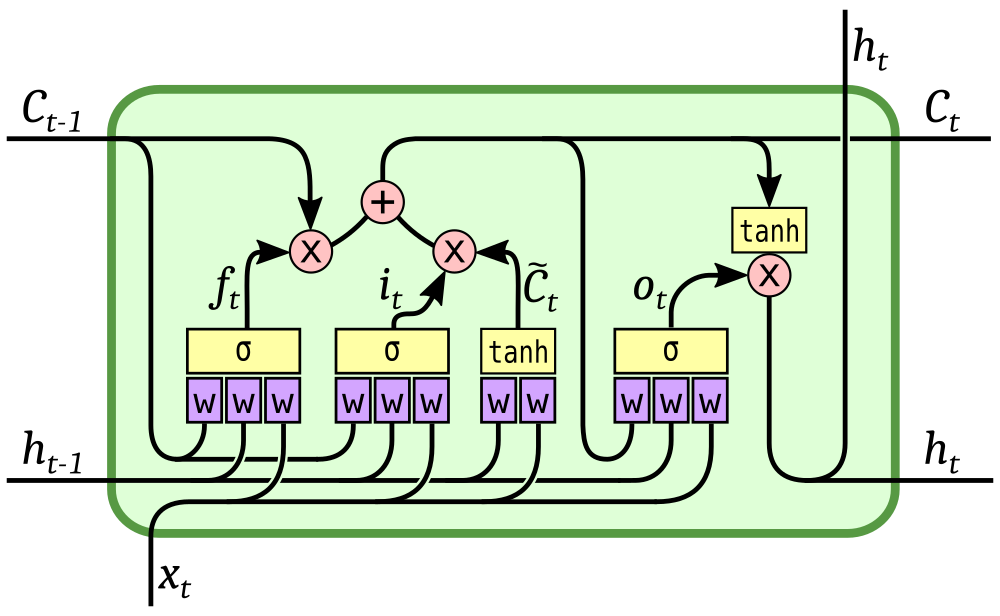
\includegraphics[width=12cm]{lstm}
    \caption{LSTM with peephole connections (Adapted from \cite{rnnplot})}
    \label{Figure:LSTM-structure}
\end{figure}

To address the vanishing/exploding gradient problem, multiple variations of RNN have been proposed. 
Long Short-Term Memory (LSTM) networks are one of the popular architectures \cite{lstm}. 
The structure of LSTM is shown in \fref{Figure:LSTM-structure}. 

The LSTM network introduces three gates to manage the weights of samples in the sequenced data. $f$ is the forget gate, $i$ is input gate, and $o$ is forget gate. 
$\sigma$ is a signoid function that gives a value between 0 and 1, which can act like a switch. 
$\mathbf{h}$ and $\mathbf{c}$ stands for hidden state and cell state. Each carries a memory path to pass down information.  
The equation of each value is given by: 

\begin{gather}
    \mathbf{i} _t=\sigma (\mathbf{w} _{xi}\mathbf{x} _t + \mathbf{w} _{hi}\mathbf{h} _{t-1} + b_i) \notag\\
    f_t=\sigma (\mathbf{w} _{xf}\mathbf{x} _t + \mathbf{w} _{hf}\mathbf{h} _{t-1} + b_f) \notag\\
    \mathbf{o} _t=\sigma (\mathbf{w} _{xo}\mathbf{x} _t + \mathbf{w} _{ho}\mathbf{h} _{t-1} + b_o) \notag\\
    \mathbf{\tilde{c} } _t=\tanh (\mathbf{w} _{xc}\mathbf{x} _t + \mathbf{w} _{hc}\mathbf{h} _{t-1} + b_c) \\
    \mathbf{c} _t=f_t \odot \mathbf{c} _{t-1} + \mathbf{i} _t \odot \mathbf{\tilde{c} } _t \notag\\
    \mathbf{h} _t=\mathbf{o} _t \odot \tanh (\mathbf{c} _t) \notag
\end{gather}

These gates, or rather sigmoid functions, let LSTM choose to ignore a sample if the current sample has been considered as not important. 
Otherwise, the LSTM will discard the information before the sample, and only retain the information of current time $t$. 

In the first version of LSTM, there is no output gate \cite{ribeiro2020exploding}, and the equations looks like this: 

\begin{gather}
    \mathbf{i} _t=\sigma (\mathbf{w} _{xi}\mathbf{x} _t + \mathbf{w} _{hi}\mathbf{h} _{t-1} + b_i) \notag\\
    f_t=\sigma (\mathbf{w} _{xf}\mathbf{x} _t + \mathbf{w} _{hf}\mathbf{h} _{t-1} + b_f) \notag\\
    \mathbf{\tilde{h} } _t=\tanh (\mathbf{w} _{xc}\mathbf{x} _t + \mathbf{w} _{hc}\mathbf{h} _{t-1} + b_c) \\
    \mathbf{h} _t=f_t \odot \mathbf{h} _{t-1} + \mathbf{i} _t \odot \mathbf{\tilde{h} } _t \notag
\end{gather}

It is clearer that in this set of equations, $\mathbf{i}$ controls the weight of short-term memories, and $f$ controls longer memories. 
Those two gates are independent. While training, it can find suitable parameters for $\mathbf{i}$ and $f$, 
which means $\mathbf{i}$ and $f$  will use different $\mathbf{x} _t$ and $\mathbf{h} _{t-1}$ to give different control strategies.

The addition of the output gate and use of $\mathbf{c}$ is to keep the longer memories more effectively. 
$\mathbf{c}$ does not exit the output gate, hence it is not affected if the current output gate is approaching 0. 
Even though the current $f$ is tend to 0, which means $\mathbf{c}_{t-1}$ has been forgotten, $\mathbf{h} _{t-1}$ still contains information about $\mathbf{c}_{t-1}$. 
This allows the long-term memories to pass down through the time sequence. 

%% ----------------------------------------------------------------
%% DataPreparation.tex
%% ---------------------------------------------------------------- 
\chapter{Data Preparation} \label{Chapter:DataPreparation}

\section{Dataset Explained}

The dataset was found and downloaded on the internet \cite{Dataset}, which is real data gathered in the city of Guiyang.
It contains both static and dynamic data throughout the years of 2015-2017, separated into three sets.

The first datasheet contains the information of a total of 132 links, the structure is shown in \fref{Figure:link_info}.
link\_ID is a string of unique IDs for each link; the length and width of the links are double values in meters; 
link\_class is the classification of the road, but since all the links in this data set are in class 1, this column has been eliminated for further processing.

\begin{figure}[!htb]
    \centering
    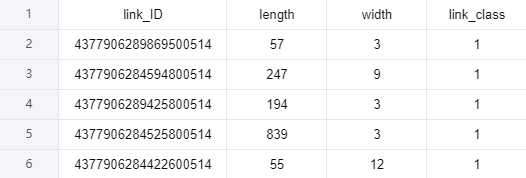
\includegraphics[width=10cm]{link info}
    \caption{First few samples of link info}
    \label{Figure:link_info}
\end{figure}

The second datasheet records the upstream and downstream relations of each link, forming the topology of the map. The structure is shown in \fref{Figure:link_top}.

\begin{figure}[!htb]
    \centering
    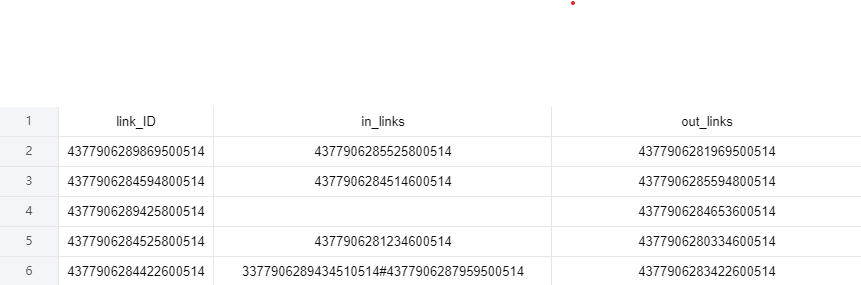
\includegraphics[width=14cm]{link top}
    \caption{First few samples of link topology}
    \label{Figure:link_top}
\end{figure}

The third datasheet is the records of the travel\_time (i.e. the average time of vehicles stays on the link) every two minutes (\fref{Figure:records}). 
A higher value of travel\_time means it takes a longer time for vehicles to pass the link, which implies the road is more congested. Hence, it is the value to predict. 
The datasheet also includes the record time interval and the date, including year and month, of the record. There are a total of 25,999,606 records, distributed mainly from March to June of 2016 and 2017.

\begin{figure}[!htb]
    \centering
    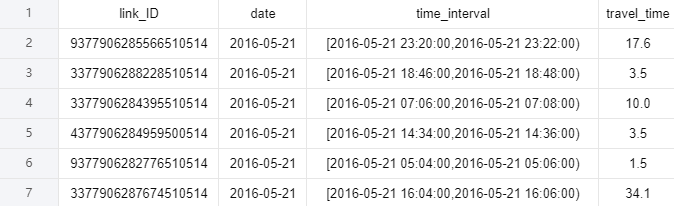
\includegraphics[width=12cm]{records}
    \caption{First few samples of records}
    \label{Figure:records}
\end{figure}

\section{Data Preparation and Evaluation}

Before the training of the model, the data needs to be analyzed first. For the RNN-based model, the data should be sorted in the sequence of time. 
With this implemented, the feature of time itself will not give much further characteristics, hence digging of the data to get more key features is vital before the training. 
This would potentially help to reach a better performance.

\subsection{Static Data}

\begin{figure}[!htb]
    \centering
    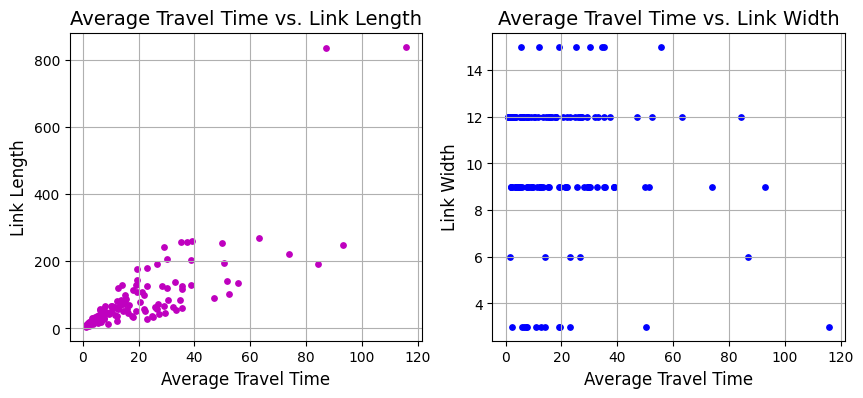
\includegraphics[width=12.5cm]{length_width_plot}
    \caption{Length \& Width vs. Average Travel Time}
    \label{Figure:length_width}
\end{figure}


The relation of the length and width of the links and the travel time has been studied, and the plot is shown in \fref{Figure:length_width}.
We can see that length has a strong positive correlation with travel time, whereas width seems not relevant at all. 

The upstream and downstream of links also are vital for prediction. It is planned to take them into account in the future. 

\subsection{Records}

The time indication features i.e. years, months, etc. are integer encoded. This might lead to the model incorrectly assuming magnitude relationships between categories. 
To eliminate this misunderstanding, one-hot encoding is used. The year contains only 2016 and 2017, which can be represented by 0 and 1, using one dimension of a sample.
The month includes every month from March to July, a total of 5 months, and five dimensions are occupied.

\begin{figure}[!htb]
    \centering
    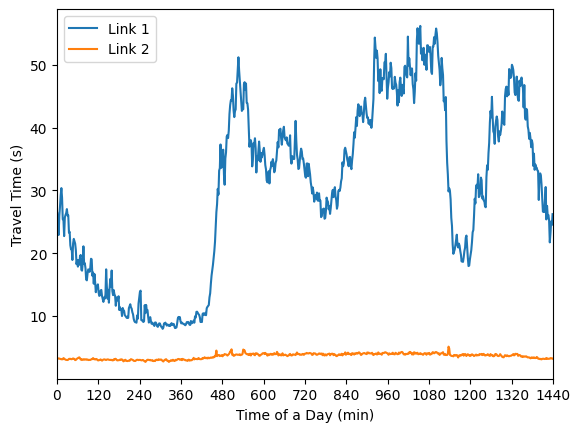
\includegraphics[width=8cm]{time of day}
    \caption{Time of day vs. average travel time of two randomly choosed links}
    \label{Figure:time_of_day}
\end{figure}

The time of the day also reveals characteristics for some of the links. \fref{Figure:time_of_day} shows the plot of two randomly chosen links.
Link1 varies a lot at different times. In contrast, Link2 gives a much flattened curve. Hour of day is decided to use as a feature, 
since it is also discrete, one-hot encoding is implemented. 

Whether it is a holiday also affects people's behaviour. Hence it would be reasonable to add a feature to tell if it is a holiday. 
Weekdays are also identified since some of the samples reveal periodicity throughout the week. 
By plotting them with the travel time on \fref{Figure:weekday_holiday}, it can be seen that the weekdays are generally higher in terms of travel time than holidays and weekends.

\begin{figure}[!htb]
    \centering
    \subcaptionbox{Holiday (1); Working day (0)}{
        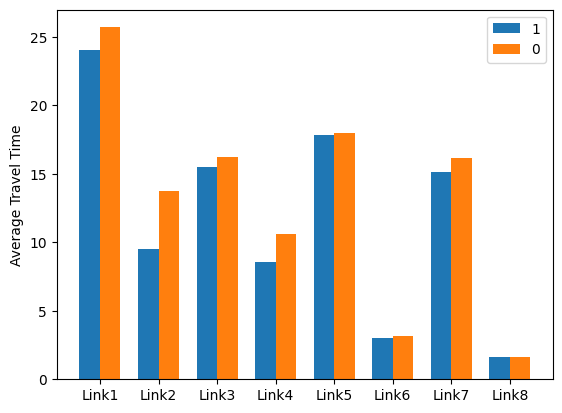
\includegraphics[width=7cm]{is holiday}
        \label{Figure:weekday_holiday:holiday}
    }
    \subcaptionbox{Weekend (1); Weekday (0)}{
        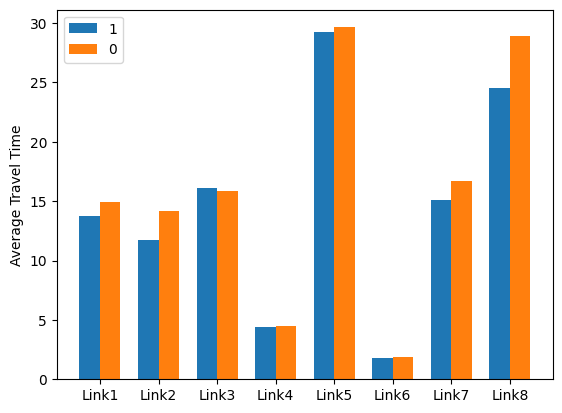
\includegraphics[width=7cm]{is weekend}
        \label{Figure:weekday_holiday:weekday}
    }
    \caption{8 randomly choosed links are used to compare (A) holiday (B) weekend with normal working day}
    \label{Figure:weekday_holiday}
\end{figure}

With everything above done, the data now have a dimension of 72 for each link. The structure is shown in \tref{Table:Dimensions}. 
There are 132 different links, each link is trained separately. 

\begin{table}[!htb]
    \centering
    \begin{tabular}{c|cc|c|cc}
    \toprule
    & length & type & & length & type \\
    \midrule
    year & 1 & bool & is\_holiday & 1 & bool \\
    month & 5 & bool & is\_weekend & 1 & bool \\
    weekday & 7 & bool & width & 1 & int \\
    day\_of\_month & 31 & bool & length & 1 & int \\
    hour\_of\_day & 24 & bool & speed & 1 & float \\
    time\_of\_day & 1 & int & travel\_time & 1 & float \\
    \bottomrule
    \end{tabular}
    \caption{Dimensions of samples for a single link}
    \label{Table:Dimensions}
\end{table}

It has been noticed that most links have missing data at various time segments.
Therefore, multiple methods were attempted to fill in the missing values. For the case where the missing values are sparse, i.e. two 
time segments before and after the sample are not missing, 
the average of the two segments before and after is used to fill in the gap. 
For large chunks of missing, drop the chunk in the training set, and fill the mean of the data of historical simultaneous moments in the test set. If fill the training set, it may cause large errors.

%% ----------------------------------------------------------------
%% DesignImplementation.tex
%% ---------------------------------------------------------------- 
\chapter{Design \& Implementation} \label{Chapter:DesignImplementation}

To implement the neural network, a deep learning library is needed. Tensorflow with Keras API is chosen. 
\aref{Appendix:listing} shows the code to implement the LSTM model.

\begin{figure}[!htb]
    \centering
    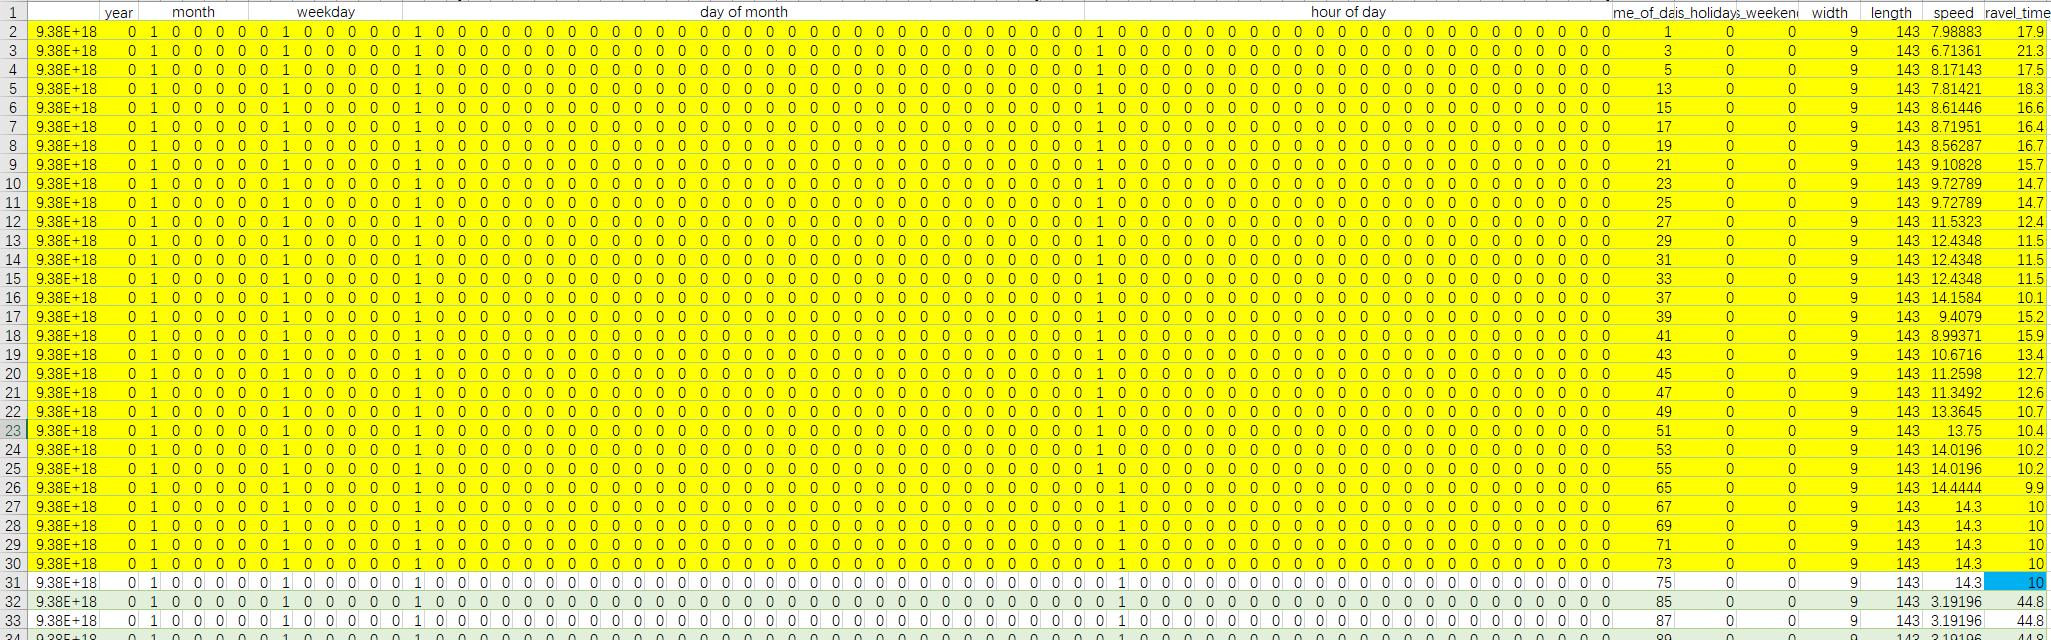
\includegraphics[width=14.5cm]{input shape}
    \caption{Yellow represents input structure; blue is the label as target}
    \label{Figure:input_shape}
\end{figure}

It is decided that to predict one sample, data from the previous 1 hour is used. For each sample, this gives an input shape of [30, 75], 30 being the previous 30 samples and 75 being the number of features.
Output shape is [1] since only the travel time will be predicted. \fref{Figure:input_shape} represents an example of one pair of inputs. 

The data have then been normalized, shuffled, and separated into training and validation sets, and it is ready to be fed into the model. The separation rate has been set to 0.9. 

\begin{figure}[!htb]
    \centering
    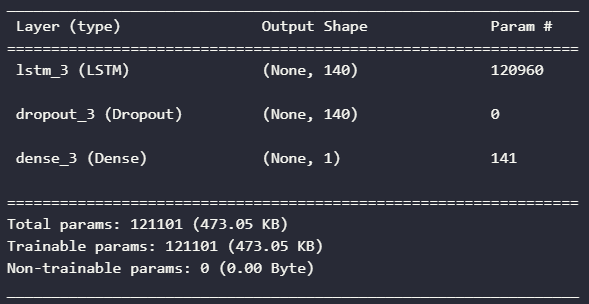
\includegraphics[width=12cm]{model_structure}
    \caption{A LSTM model constructed using Keras}
    \label{Figure:model_structure}
\end{figure}

A one-layer LSTM model is constructed, with a dropout layer of 0.2 and a dense layer, shown in \fref{Figure:model_structure}.

After 70 epochs, the model reaches its point of early stopping, with an MSE loss of $6.17\times 10^{-4}$. 

\begin{figure}[!htb]
    \centering
    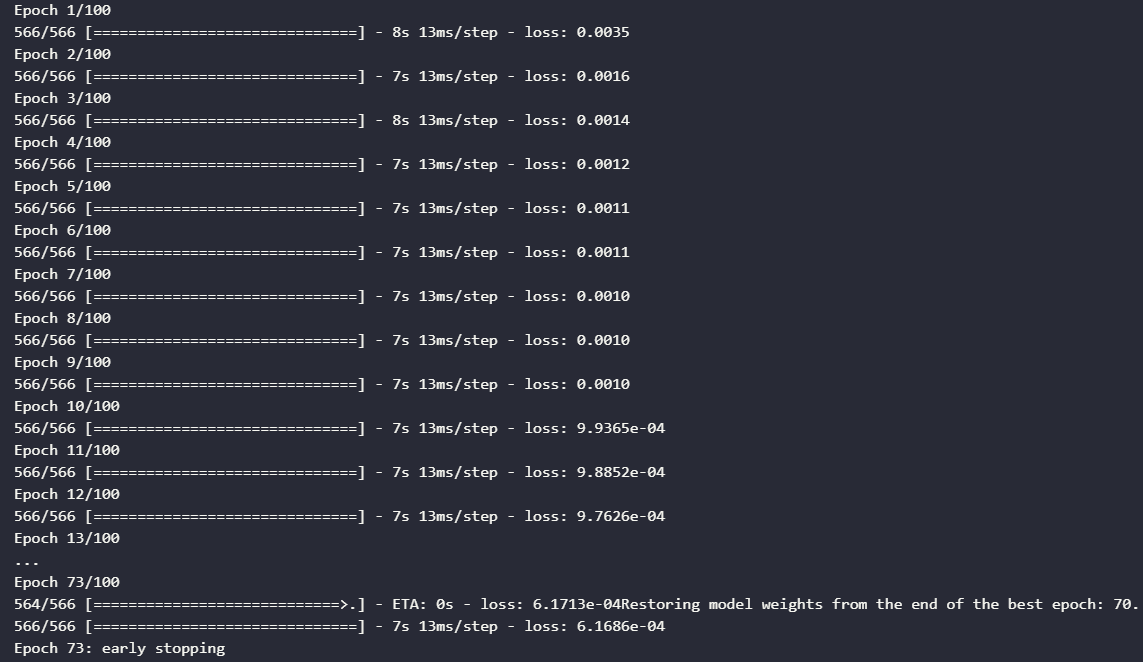
\includegraphics[width=12cm]{result1}
    \caption{Result}
    \label{Figure:result1}
\end{figure}

A plot of predicted value vs. target value is shown in \fref{Figure:result1_plot}. For this plot, the closer the points to the line $y = x$, the better the prediction is. 

\begin{figure}[!htb]
    \centering
    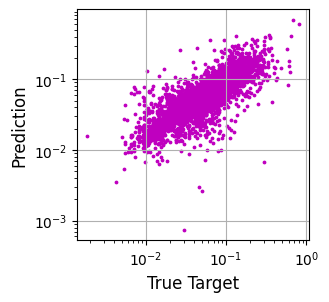
\includegraphics[width=8cm]{result validation}
    \caption{Predicted vs. target value}
    \label{Figure:result1_plot}
\end{figure}


%% ----------------------------------------------------------------
%% Conclusions.tex
%% ---------------------------------------------------------------- 
\chapter{Conclusions \& Proposal} \label{Chapter: Conclusions}

\section{Conclusions}

A Gantt Chart of all the work done is shown in \aref{Appendix:listing}, \fref{Figure:gantt}.
Up to this point, the background of the LSTM model has been well-researched. The dataset has been found, and the data are well understood. 
Several method to preprocess the data in temporal aspects has been go through, to reconstruct a better dataset fed into the model. 
A simple LSTM model has been built, given a basic working skeleton of this project. 

\section{Future Work}

The chart also states the work not completed and planned to be done in the future.

The deep learning library still needs to be more familiarized. It is the priority to have a better structure for the network 
by altering the number of LSTM layers, batch sizes, and so on. These hyperparameters could be optimised using Bayesian optimisation. 

The information on upstream and downstream has not been used for now, consider using spatio-temporal graph convolutional networks (STGCN) method \cite{DBLP:journals/corr/abs-1709-04875}\cite{8560205} to extract 
traffic's spatial characteristics as well, to potentially reach better performance. Hence, further background research on Bayesian optimisation and STGCN is required. 

The LSTM model is sensitive to missing values, consider the LSTM-M model \cite{TIAN2018297} to reduce its impact.

A navigation algorithm based on the A* method will be implemented to show how the model can benefit daily lives. 

%% ------------------ BACK MATTER ORGANISATION -------------------

\bibliographystyle{plainnat}
\bibliography{UOS}

\appendix
%% ----------------------------------------------------------------
%% AppendixA.tex
%% ---------------------------------------------------------------- 
\chapter{Listings} \label{Appendix:listing}

\begin{lstlisting}[caption=Code of the LSTM model's skeleton]
def normalize(vector):
    scaler = preprocessing.MinMaxScaler()
    return scaler.fit_transform(vector)

def sort_samples_by_link(data):
    sorted_data = {}
    for record in data:
        if record[0] in sorted_data.keys():
            sorted_data[record[0]].append(record[1:])
        else: sorted_data[record[0]] = [record[1:]]
    return sorted_data

def create_inout_sequences(data, shape):
    x = np.zeros((data.shape[0]-shape[0], shape[0], shape[1]))
    y = np.zeros((data.shape[0]-shape[0], 1))
    for i in range(data.shape[0]-shape[0]):
        train_seq = data[i:i+shape[0]]
        train_lbl = data[i+shape[0]:i+shape[0]+1][0][-1]
        x[i] = train_seq
        y[i] = train_lbl
    return x, y

ExpandedDataLoaded = sort_samples_by_link(load_expanded_data())
useData = np.array(ExpandedDataLoaded['4377906280329500514']) # Use one link

useData[:, 68] = normalize(useData[:, 68].reshape(-1, 1)).reshape(1, -1)
useData[:, 71:] = normalize(useData[:, 71:])

x, y = create_inout_sequences(useData, [30, 75])
X_train, X_test, y_train, y_test = train_test_split(x, y, test_size=0.1, 
                                                    shuffle=True)
model = Sequential()
earlystop = EarlyStopping(monitor='loss', min_delta=0, 
                            patience=3, verbose=1, restore_best_weights=True)
model.add(LSTM(units=140, return_sequences=False, 
                input_shape=(X_train.shape[1], X_train.shape[2])))
model.add(Dropout(0.2))
model.add(Dense(units=10, activation='sigmoid'))
model.compile(optimizer='adam', loss=tf.keras.losses.MeanSquaredError())
model.summary()

model.fit(X_train, y_train, epochs=100, batch_size=100, callbacks=earlystop)
\end{lstlisting}

\chapter{Charts} \label{Appendix:chart}

\begin{figure}[!htb]
    \centering
    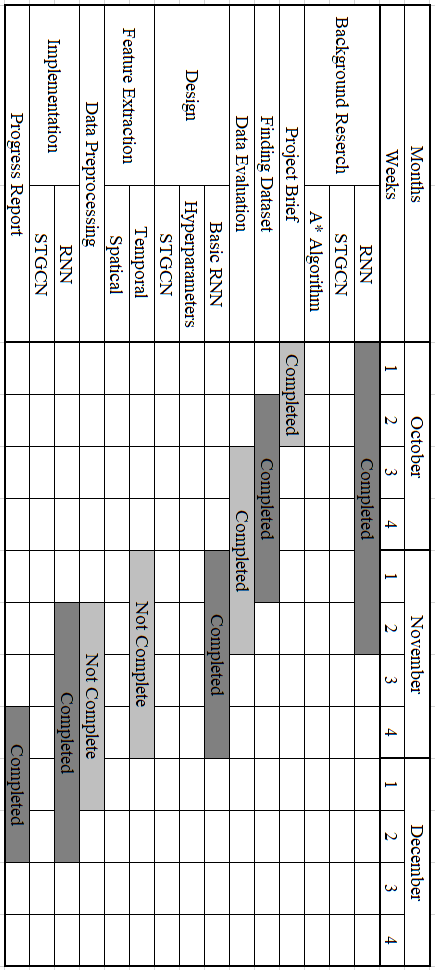
\includegraphics[width=7.8cm]{Gantt Chart}
    \caption{Gantt Chart}
    \label{Figure:gantt}
\end{figure}

\backmatter

% \chapter{Glossary [if relevant]}

% \chapter{Bibliography}
% To use bibliography as well as the references section use the \texttt{multibbl} package.

% \chapter{Index [if relevant]}

\end{document}
%% ----------------------------------------------------------------
